
\begin{center}
\Huge
Geometrisk løsning af andengradsligninger
\end{center}
\stepcounter{section}
Vi husker på, at en andengradslignings er en ligning på formen
\begin{align*}
ax^2+bx+c=0,
\end{align*}
hvor $a,b,c\in \mathbb{R},a\neq 0.$ Disse kan generelt løses med diskriminantformlen
\begin{align*}
x = \frac{-b\pm \sqrt{b^2-4ac}}{2a}.
\end{align*}
Dette giver os selvfølgelig en metode til at løse ligningen algebraisk, men det giver ikke meget intuition i forhold til hvad det rent faktisk er, vi løser. Som i så mange andre grene af matematik er der en række forskellige synspunkter, hvor det mest udbredte er at se løsningen til andengradsligninger som nulpunkter/rødder af en bestemt type funktioner. Vi fastlægger først, hvad vi mener med en rod/et nulpunkt.
\begin{defn}
Vi siger, at et punkt $x$ er en rod for en funktion $f$, hvis det gælder, at $f(x)=0$. Rødder kaldes også for nulpunkter. 
\end{defn}
\begin{defn}
En funktion på formen $f(x)=ax^2+bx+c$ for $a,b,c\in \mathbb{R},\ a \neq 0$ kaldes for et andengradspolynomium. Grafen for et andengradspolynomium kaldes for en parabel.
\end{defn}
Det ses let, at det at finde rødder til et andengradspolynomium tilsvarer at løse en andengradsligning. 
\begin{exa}
Vi betragter andengradspolynomiet $f(x) = x^2-x-2$. Grafen for $f$ kan ses af Fig. \ref{fig:andengp}
\begin{figure}[H]
\center
\begin{tikzpicture}
\begin{axis}[axis lines=middle,
xtick ={-5,-4,...,5},
xmin= -6,xmax=6,
ymin=-5,ymax=10,
xlabel = {$x$},
ylabel = {$y$},
]
\addplot[color=blue!40,thick,samples=1000]{x^2-x-2};
\end{axis}
\end{tikzpicture}
\caption{Parabel, der er graf for andengradspolynomiet $f(x)=x^2-x-2$.}
\label{fig:andengp}
\end{figure}
At finde rødderne for $f$ tilsvarer at finde de punkter, hvor grafen for $f$ skærer $x$-aksen. Af Fig. \ref{fig:andengp} ser det ud til, at $f(x)$ har rødder i $x=-1$ og $x=2$. Vi tjekker efter og får
\begin{align*}
f(-1) &= (-1)^2+1-2 = 1+1-2=0,\\
f(2) &= 2^2-2 - 2  = 4-2-2 = 0.
\end{align*}
Derfor har andengradsligningen $x^2-x-2=0$ løsningerne $x=-1$ og $x=2$.
\end{exa}
Vi husker på, at andengradsligninger enten har 0, 1 eller 2 løsninger. Dette tilsvarer at parablen til andengradspolynomiet skærer $x$-aksen enten 0, 1 eller 2 gange som vist på Fig. \ref{fig:3parabler}.
\begin{figure}[H]
\center
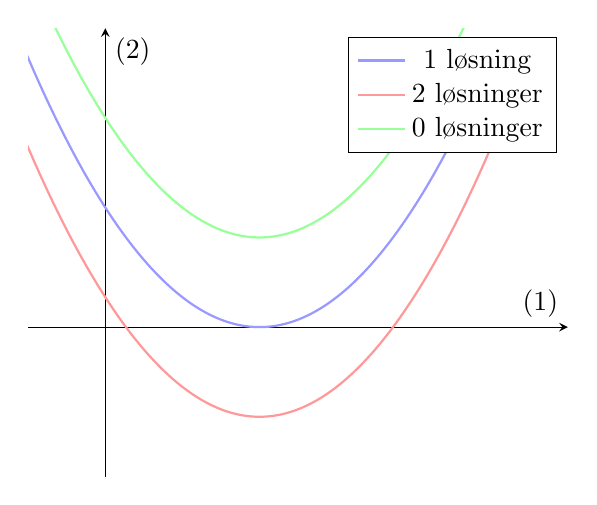
\begin{tikzpicture}
\begin{axis}[axis lines=middle, ticks = none,
xmin= -1,xmax=6,
ymin=-5,ymax=10,
xlabel = {$(1)$},
ylabel = {$(2)$},
]
\addplot[color=blue!40,thick,samples=1000]{x^2-4*x+4};
\addplot[color=red!40,thick,samples=1000]{x^2-4*x+1};
\addplot[color=green!40,thick,samples=1000]{x^2-4*x+7};
\legend{1 løsning, 2 løsninger, 0 løsninger}
\end{axis}
\end{tikzpicture}
\caption{De tre muligheder for antallet af løsninger af andengradsligninger.}
\label{fig:3parabler}
\end{figure}
Vi kan udnytte dette til at afgøre, hvor mange løsninger en andengradsligning har ved at skitsere det tilsvarende andengradspolynomium. Til dette vil vi udnytte, hvad koefficienterne $a,b$ og $c$ betyder for et andengradspolynomium:
\begin{setn}
For koefficienterne $a,b,c$ for et andengradspolynomium gælder der:
\begin{enumerate}[label=\roman*)]
\item $a>0$ medfører, at parablens "arme" peger op. $a<0$ medfører, at parablens "arme" peger ned.
\item $b$ er hældningen af parablem der hvor parablen skærer $y$-aksen.
\item $c$ er parablens skæring med $y$-aksen. 
\end{enumerate}
\end{setn}
\begin{exa}
Vi kan skitsere parablen for polynomiet $f(x) = x^2-x-6$. Da $a=1>0$, så peger armene op. Da $b=1$, så er hældningen af funktionen $1$, der hvor $f$ skærer $y$-aksen. Parablen skærer $y$-aksen i $-6$. Vi kan derfor lave en skitse. Den kan ses på Fig. \ref{fig:parabelskitse}.
\begin{figure}[H]
\center
\begin{tikzpicture}
\begin{axis}[axis lines=middle,
xtick = {0},
ytick = {0},
extra y ticks={-6},
xmin= -5,xmax=4,
ymin=-8,ymax=10,
xlabel = {$(1)$},
ylabel = {$(2)$},
]
\addplot[color=blue!40,thick,samples=1000]{x^2+x-6};
\end{axis}
\end{tikzpicture}
\caption{Skitse af $f(x) = x^2+x-6$}
\label{fig:parabelskitse}
\end{figure}
Af Fig. \ref{fig:parabelskitse} kan vi se, at $x^2+x-6$ har to løsninger. En positiv løsning og en negativ løsning. 
\end{exa}
\section*{Opgave 1}
Skitsér følgende andengradspolynomier og afgør, hvor mange rødder de har samt røddernes fortegn:
\begin{align*}
&1) \ -2x^2+3x+5   &&2) \ 4x^2-5x-10   \\
&3) \  3x^2+x+20  &&4) \ x^2   \\
&5) \  -x^2-x+4   &&6) \ 6x^2-6x-6   \\
&7) \   -6x^2-6x-6 &&8) \ (x-2)^2   \\ 
\end{align*}